%%%%%%%%%%%%%%%%%%%%%%%%%%%%%%%%%%%%%%%%%
% Short Sectioned Assignment
% LaTeX Template
% Version 1.0 (5/5/12)
%
% This template has been downloaded from:
% http://www.LaTeXTemplates.com
%
% Original author:
% Frits Wenneker (http://www.howtotex.com)
%
% License:
% CC BY-NC-SA 3.0 (http://creativecommons.org/licenses/by-nc-sa/3.0/)
%
%%%%%%%%%%%%%%%%%%%%%%%%%%%%%%%%%%%%%%%%%

%----------------------------------------------------------------------------------------
%	PACKAGES AND OTHER DOCUMENT CONFIGURATIONS
%----------------------------------------------------------------------------------------

\documentclass[paper=a4, fontsize=11pt]{scrartcl} % A4 paper and 11pt font size

\usepackage[T1]{fontenc} % Use 8-bit encoding that has 256 glyphs
%\usepackage{fourier} % Use the Adobe Utopia font for the document - comment this line to return to the LaTeX default
\usepackage[english]{babel} % English language/hyphenation
\usepackage{amsmath,amsfonts,amsthm} % Math packages
\usepackage{mathtools} %More math! (For dscases)
\usepackage{hyperref} %HTML package
\usepackage{pgfplots} %Makes plots in LaTeX
\usepackage{tikz} %Also tikz?
\usepackage{bm} %makes vectors bold
\usepackage{bbm} %Blackboard bold 1
\usepgfplotslibrary{fillbetween}%Let's me fill between named plots
\usepackage{graphicx} %import pics

\usepackage[noend]{algpseudocode} %Algorithms
\usepackage{algorithm}

\graphicspath{ {Python\_figs/} }
\DeclareGraphicsExtensions{.pdf,.png,.jpg}
\usepackage{sectsty} % Allows customizing section commands
\allsectionsfont{ \normalfont\scshape} % Make all sections the default font and small caps


\renewcommand{\thesubsection}{\alph{subsection}} %Make subsections start with letters

\usepackage{fancyhdr} % Custom headers and footers
\pagestyle{fancyplain} % Makes all pages in the document conform to the custom headers and footers
\fancyhead{} % No page header - if you want one, create it in the same way as the footers below
\fancyfoot[L]{} % Empty left footer
\fancyfoot[C]{} % Empty center footer
\fancyfoot[R]{\thepage} % Page numbering for right footer
\renewcommand{\headrulewidth}{0pt} % Remove header underlines
\renewcommand{\footrulewidth}{0pt} % Remove footer underlines
\setlength{\headheight}{13.6pt} % Customize the height of the header

\numberwithin{equation}{section} % Number equations within sections (i.e. 1.1, 1.2, 2.1, 2.2 instead of 1, 2, 3, 4)
\numberwithin{figure}{section} % Number figures within sections (i.e. 1.1, 1.2, 2.1, 2.2 instead of 1, 2, 3, 4)
\numberwithin{table}{section} % Number tables within sections (i.e. 1.1, 1.2, 2.1, 2.2 instead of 1, 2, 3, 4)

\setlength\parindent{0pt} % Removes all indentation from paragraphs - comment this line for an assignment with lots of text
\usepackage{listings}
\lstset{language=Python}


\usepackage{tikz}
\usetikzlibrary{decorations.pathmorphing}
\usetikzlibrary{arrows}


%----------------------------------------------------------------------------------------
%	TITLE SECTION
%----------------------------------------------------------------------------------------

\newcommand{\horrule}[1]{\rule{\linewidth}{#1}} % Create horizontal rule command with 1 argument of height

\title{	Assignment 8}

\author{Benjamin Jakubowski} % Your name

\date{\normalsize\today} % Today's date or a custom date

\begin{document}

\maketitle % Print the title

%----------------------------------------------------------------------------------------
%	PROBLEM 1
%----------------------------------------------------------------------------------------
\section{Show $G$ has a unique MST}

Let $G$ be a graph where for every cut there is a unique light edge crossing the cut. We show the graph has a unique minimum spanning trees (MSTs).\\

Let $T_1$ and $T_2$ be two MSTs of $G$. Now if $T_1 \ne T_2$, there must be some $u \in V$ such that $(u, v) \in T_1$ but $(u, v) \notin T_2$. Note removing the edge $(u,v)$ from $T_1$ produces two disconnected subtrees $S_1$ and $S_2$ and defines a cut of $G$, namely $(S_1.V, V - S_1.V = S_2.V)$. Now, since $T_2$ is a tree and thus connected, there must be vertices $x$ and $y$ in $S_1$ and $S_2$, respectively, such that $(x,y) \in T_2$.
\begin{center}
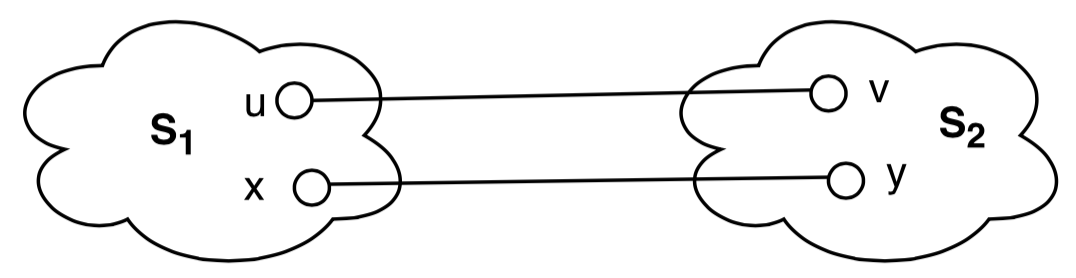
\includegraphics[scale=0.6]{figures/HW8-1.png}
\end{center}
Now, by CLRT 23.1-3, $(u,v)$ and $(x,y)$ must both be light edges since they are edges in MSTs of $G$. But then, since all light edges are unique, $(u,v) = (x,y)$. Hence $T_1 = T_2$, so $G$ has a single unique MST.

Now for the counter example to disprove the converse: the graph shown below has a unique MST but does not have a unique light edge crossing each cut.

\begin{center}
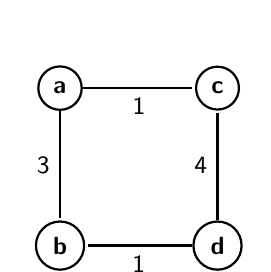
\begin{tikzpicture}[>=stealth',shorten >=1pt,auto,node distance=2cm, thick,main node/.style={circle,draw,font=\sffamily\small\bfseries}]

  \node[main node] (a) {a};
  \node[main node] (b) [below of=a] {b};
  \node[main node] (c) [right of=a] {c};
  \node[main node] (d) [below of=c] {d};
  
  \path[every node/.style={font=\sffamily\small}]
    (a) edge node [left] {3} (b)
    	 edge node [below] {1} (c)
    (d) edge node [below] {1} (b)
         edge node [left] {4} (c);
    
\end{tikzpicture}
\end{center}

%----------------------------------------------------------------------------------------
%	PROBLEM 2
%----------------------------------------------------------------------------------------

\section{Second-best MSTs}

Now let $G = (V, E)$ be an undirected, connected graph whose weight function is $w: E \to \mathbb{R}$, with $|E| \geq |V|$ and all edge weights distinct.

\subsection{MST is unique but second-best MST not necessarily unique}

Since all edge weights are distinct, for every cut of the graph $G$ there is a unique light edge. Thus by problem 1, $G$ has a unique MST.

We show the second-best MST is not necessarily unique by providing an example:

\begin{center}
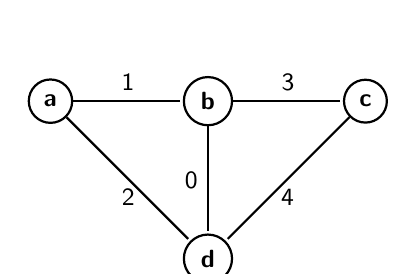
\begin{tikzpicture}[>=stealth',shorten >=1pt,auto,node distance=2cm, thick,main node/.style={circle,draw,font=\sffamily\small\bfseries}]

  \node[main node] (a) {a};
  \node[main node] (b) [right of=a] {b};
  \node[main node] (c) [right of=b] {c};
  \node[main node] (d) [below of=b] {d};
  
  \path[every node/.style={font=\sffamily\small}]
    (a) edge node [above] {1} (b)
    	 edge node [below] {2} (d)
    (b) edge node [above] {3} (c)
         edge node [left] {0} (d)
    (c) edge node [below] {4} (d);
    
\end{tikzpicture}
\end{center}

\subsection{Constructing a second-best MST}

We now show that $G$ contains $(u, v) \in T$ and $(x,y) \notin T$ such that $T - \{(u,v)\} \cup \{(x,y)\}$ is a second-best MST of $G$. \\

First note we must replace at least one edge in $T$ to obtain a second-best MST $T''$. If we didn't replace any edges, we'd have $T$, which is still our $MST$. Thus assume we replace at least one edge (noting this statement allows for replacement of all edges in $T$).\\

Now assume we can obtain a second-best MST $T''$ by replacing two or more edges. We show this yields a contradiction, and thus we must only replace a single edge to obtain our second-best MST. \\

Since we replace at least two edges, say we remove $(u_1, v_1), (u_2, v_2)$ from $T$. This produces three disconnected subtrees $S_1, S_2,$ and $S_3$. Since we are constructing our second-best MST $T''$, we must connect these components- thus we need to replace $(u_1, v_1), (u_2, v_2)$ with two of $(x_1, y_1), (x_2, y_2), $ and $(x_3, y_3)$.
\begin{center}
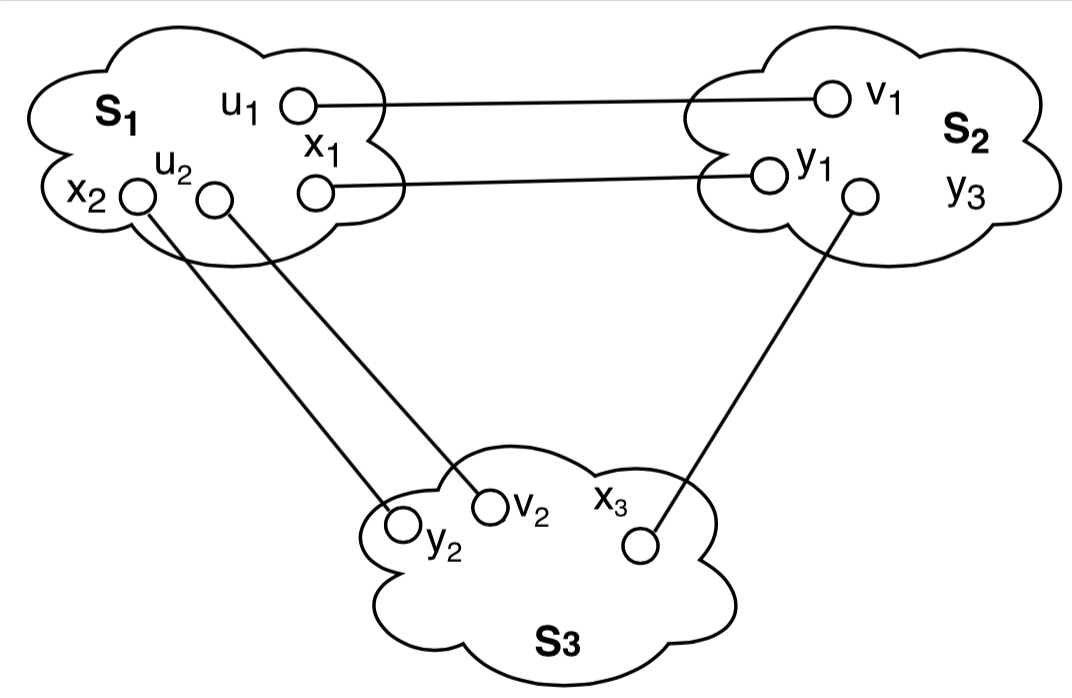
\includegraphics[scale=0.6]{figures/HW8-2breal.png}
\end{center}

In particular note that we must have either
\begin{itemize}
\item Cut $(u_1, v_1)$ and pasted $(x_1, y_1)$. In this case, note since $T$ was our MST, $w(u_1, v_1) < w(x_1, y_1)$. 
\item  Cut $(u_2, v_2)$ and pasted $(x_2, y_2)$. In this case, similarly note since $T$ was our MST, $w(u_2, v_2) < w(x_2, y_2)$. 
\end{itemize}

Without loss of generality, let's say we cut $(u_1, v_1)$ and pasted $(x_1, y_1)$ (the second case is identical, so we address just the first case to ease notation). Then note we can construct a new spanning tree $T'''$ by undoing this cut-and-paste (replacing $(x_1, y_1)$ in $T''$ with $(u_1, v_1)$). Now, since $w(u_1, v_1) < w(x_1, y_1)$, $w(T''') < w(T'')$. However, $T''' \ne T$. Thus we have
\[w(T) < w(T''') < w(T'')\]

But then we have our contradiction, namely that $T''$ is not a second-best MST. Instead $T'''$ is our second-best MST. Thus we only replace a single edge from $T$ to construct our second-best MST.

\subsection{$O(V^2)$ algorithm to compute $\max [u,v]$}

Now let $T$ be a spanning tree of $G$ and, for any two vertices $u, v \in V$ let $\max[u, v]$ denote an edge of maximum weight on the unique simple path between $u$ and $v$ in $T$. We present an $O(V^2)$-time algorithm that, given $T$, computes $\max[u,v]$ for all $u, v \in V$. 

\begin{algorithmic}
\Function{find\_max}{T}
	\For {$v \in G.V$}
		\State modified\_BFS(T, v)
	\EndFor
\EndFunction
\end{algorithmic}

The bulk of the work is clearly in \texttt{modified\_BFS}(T, v). This helper function runs a breadth first search from v, with the modification being the computation and storage of the maximum weight in the path from s to every other vertex in the tree.\\

\begin{algorithmic}[1]
\Function{modified\_BFS}{T, s}
	\For {$v \in G.V - \{s\}$}
		\State v.color = white
		\State v.d = $\infty$
		\State v.$\pi$ = NIL
		\State v.max[s] = $- \infty$ \Comment{v.max[s] stores max weight in path from $v$ to $s$}
	\EndFor
	\State s.color = Gray
	\State s.d = 0
	\State s.$\pi$ = NIL
	\State s.max[s] = $- \infty$
	\State Q = new Queue
	\State Enqueue(Q, s)
	\While {Q is not empty}
		\State u = Dequeue(Q)
		\For {each $v \in G.Adj[u]$}
			\If{v.color == white}
				\State v.color = gray
				\State v.d = u.d + 1
				\State v.$\pi$ = u
				\If {w(u,v) > u.max[s]}
					\State v.max[s] = w(u,v)
					\State v.max\_edge[s] = (u,v)
				\Else
					\State v.max[s] = u.max[s]
					\State v.max\_edge[s] = u.max\_edge[s]
				\EndIf
				\State Eunqueue(Q,v)
			\EndIf
		\EndFor
		\State u.color = black
	\EndWhile
\EndFunction
\end{algorithmic}

Obviously the additional steps in \texttt{modified\_BFS} (lines 6, 10, and 20-25) are constant time additions to BFS. Hence the time complexity of \texttt{modified\_BFS} is still just $O(V + E)$. However, since we're restricting our search to trees, $|E| = |V| - 1$, so \texttt{modified\_BFS} is just $O(V)$. Since we call this function $|V|$ times, our algorithm is $O(V^2)$ as desired.

\subsection{Algorithm to compute the second-best MST of $G$}

Finally, we present an algorithm to compute the second-best MST of $G$. The basic idea of the algorithm is to
\begin{itemize}
\item Compute the unique MST $T$
\item Find the edge $(u,v)$ not in $T$ such that removing the maximum weight edge in the path between $u$ and $v$ in $T$ and adding $(u,v)$ increases the weight the least.
\item Return this second best spanning tree.
\end{itemize}

\begin{algorithmic}[1]
\Function{find\_second\_best\_MST}{T, s}
	\State T = minimum\_spanning\_tree(G, w) \Comment{Using Kruskal or Prim}
	\State find\_max(T) \Comment{Annotates tree with max weight edge between each $u, v$}
	\State min\_diff = $\infty$
	\For {(u,v) $\in$ G and $\notin$ T.E}
		\If {w(u,v) - u.max[v] < min\_diff}
			\State edge\_to\_add = (u,v)
			\State edge\_to\_delete = u.max\_edge[v]
		\EndIf
	\EndFor
	\State T'' = T.E - edge\_to\_delete $\cap$ edge\_to\_add
	\State \Return T''
\EndFunction
\end{algorithmic}

To analyze the runtime of this algorithm, note
\begin{itemize}
\item On line 2 we can compute the spanning tree in $O(E \lg V)$
\item On line 3 running find\_max on tree T is $O(V^2)$
\item Assuming the lookups needed on lines 6-8 are constant time, the for loop on lines 5-8 run in $O(E - V)$ (since we check every edge not in the tree, and there are $V-1$ edges in the tree).
\end{itemize}

%----------------------------------------------------------------------------------------
%	PROBLEM 3
%----------------------------------------------------------------------------------------

\section{Most reliable path}

Let $G = (V,E)$ be a directed graph on which each edge is an associated value $r(u,v) \in [0,1]$, which we interpret as the probability that the channel from $u$ to $v$ will not fail. Assume that the probabilities are independent. We present an efficient algorithm to find the most reliable path between two given vertices.\\

First, consider a path between $v_0 \sim v_k$, where $v_0 \sim v_k = \langle v_0, v_1, v_2, \cdots, v_k \rangle$. Then by independence
\[P(\textrm{Probability successful communication between } v_0 \textrm{ and } v_k) = \prod_{i = 0}^{k-1} r(v_i, v_{i+1})\]

Now note we aim to find
\begin{align*}
v_0 \stackrel{*}{\sim}v_k &= \arg \max_{\{v_0 \sim v_k} \prod_{i = 0}^{k - 1} r(v_i, v_{i+1}) \\
	 &= \arg \min_{\textrm{All paths }v_0 \sim v_k} - \log[\prod_{i = 0}^{k - 1} r(v_i, v_{i+1})] \\
	 &= \arg \min_{\textrm{All paths }v_0 \sim v_k} - \sum_{i = 0}^{k - 1}\log\left(r(v_i, v_{i+1})\right) \\
\end{align*}
where we let $k$ be the length of the path under consideration (i.e. a variable, not constant). \\

But now this is a problem amenable to our standard algorithms- since $-\log(x) \geq 0$ for all $x \in (0, 1]$, we can just use Dijkstra's. Thus the final algorithm is just\\

\begin{algorithmic}
\Function{most\_reliable\_path}{G, u, v}
	\For {$(u',v')$ in G.E}
		\If {$r(u',v') = 0$}
			\State delete $(u',v')$ \Comment{Edge not in any reliable path}
		\Else
			\State $r(u',v') = -\log r(u',v')$
		\EndIf
	\EndFor
	\State \texttt{Dijkstra}$(G, -\log r, u)$
	\State \Return v.d
\EndFunction
\end{algorithmic}

%----------------------------------------------------------------------------------------
%	PROBLEM 4
%----------------------------------------------------------------------------------------

\section{Nesting boxes}

A $d$-dimensional box with dimensions $(x_1, x_2, \cdots, x_d)~nests$ within another box with dimensions $(y_1, y_2, \cdots, y_d)$ if there exists a permutation $\pi$ on $\{1, 2, \cdots, d\}$ such that $x_{\pi(1)} < y_1, \cdots, x_{\pi(d)} < y_d$.

\subsection{Nesting relation is transitive}

We first show the nesting relation is transitive. Say $x$ nests in $y$, and $y$ nests in $z$. We show $x$ nests in $z$.

Since $y$ nests in $z$, there exists some $\pi_{yz}$ such that $y_{\pi_{yz}(1)} < z_1, \cdots, y_{\pi_{yz}(d)} < z_d$. \\

Similarly, $x$ nests in $y$, there exists some $\pi_{xy}$ such that $x_{\pi_{xy}(1)} < y_1, \cdots, x_{\pi_{xy}(d)} < y_d$. \\

But then composing the permutation $\pi_{yz}$ and $\pi_{xy}$ yields a permutation such that

\[x_{\pi_{xy}\left(\pi_{yz}(1)\right)} < z_1, \cdots, x_{\pi_{xy}\left(\pi_{yz}(d)\right)} < z_d\]

Hence $nesting$ is a transitive relation.

\subsection{Efficient method to determine whether or not one box nests inside another}

First, note that a box $x$ nests inside a box $y$ if there is relative ordering of the dimensions of x and y such that
\[x_{\pi(i)} < y_i \qquad{} \forall ~ i \in \{1, \cdots, d\}\]

Clearly such a permutation exists if and only if
\[\textrm{sorted}(x)_{i} < \textrm{sorted}(y)_{i} \qquad{} \forall ~ i \in \{1, \cdots, d\}\]

Thus, a linearithmic algorithm to see if $x$ nests in $y$\ is \\

\begin{algorithmic}
\Function{boxes\_nest}{$y,x$}
	\State sort $x$ \Comment{using your favorite linearithmic sorting algorithm}
	\State sort $y$
	\For {$i$ in 1 to $d$}
		\If {$x_i \geq y_i$}
			\State \Return false 
		\EndIf
	\EndFor
	\State \Return true
	\EndFunction
\end{algorithmic}

\subsection{Finding longest sequence of nesting boxes}

Now suppose we are given a set of $n$ $d$-dimensional boxes $\{B_1, \cdots, B_n\}$. We present an algorithm to find the longest sequence $\langle B_{i_1}, \cdots, B_{i_k}\rangle$ of boxes such that $B_{i_j}$ nests within $B_{i_{j+1}}$ for $j = 1, 2, \cdots, k-1$. \\

We first present a couple of helper function to sort the set of boxes. To briefly motivate \texttt{sort\_boxes}, note this function (i) sorts the dimensions of each box in increasing order, then (ii) sorts the set of boxes in decreasing order of smallest dimension. Sort (ii) reveals the pairs of boxes $B_i, B_j$ that do not nest; namely, if $i < j$, then $B_i$ does not nest in $B_j$. \\

The second helper function \texttt{sorted\_boxes\_nest} just refactors \texttt{boxes\_nest} to avoid duplicating the sorting step.

\begin{algorithmic}
\Function{sort\_boxes}{$\{B_1, \cdots, B_n\}$}
	\For {i in 1 to n}
		\State sort $B_i$
	\EndFor
	sort $\{\textrm{sorted}(B_1), \cdots, \textrm{sorted}(B_n)\}$ by smallest dimension in decreasing order
\EndFunction
\end{algorithmic}

\begin{algorithmic}
\Function{sorted\_boxes\_nest}{$x,y$}
	\For {$i$ in 1 to $d$}
		\If {$y_i \geq x_i$}
			\State \Return false 
		\EndIf
	\EndFor
	\State \Return true
	\EndFunction
\end{algorithmic}

Now that we've presented the helper functions, we present the actual algorithm. Note following the call to \texttt{sort\_boxes}, we ease notation by letting $B_i$ be the $i^{th}$ box in sorted order. The algorithm proceeds by constructing a weighted DAG, where the edge $(B_i, B_j)$ indicates $B_j$ nests inside $B_i$. We assign each edge a weight of $-1$, since this will allow us to find the longest path through the DAG beginning at the super source using standard shortest-path algorithms (since the longest path with have the least weight).

\begin{algorithmic}[1]
\Function{longest\_nested\_sequence}{$\{B_1, \cdots, B_n\}$}
	\State sort\_boxes($\{B_1, \cdots, B_n\}$)
	\State $E = \{super\}$
	\State $V = \{\}$
	\State $G = \{E,V\}$
	\For {$i$ in 1 to $n$}
		\State $V = V \cup \{B_i\}$
		\State $E = E \cup \{(super, B_i)\}$
		\State $w((super, B_i)) = -1$
		\For {$j$ in $i + 1$ to $n$} \Comment {After sorting, no $B_k$ with $k < i$ nests inside $B_i$}
			\If {sorted\_boxes\_nest($B_i, B_j$)}
				\State $E = E \cup \{(B_i, B_j)\}$
				\State $w((B_i, B_j)) = -1$
			\EndIf
		\EndFor
	\EndFor
	\State DAG-SHORTEST-PATHS($G, w, super$)
	\State \Return - min($B_i$.d) for $i$ in 1 to $n$ \Comment{Longest path through DAG from $super$}
	\EndFunction
\end{algorithmic}

Now we analyze the running time:
\begin{itemize}
\item First, on line 2 sorting all of the $n$ boxes takes $O(d ~ n \lg n)$ time, and sorting the $n$ boxes in decreasing order of their smallest dimension takes $O(n \lg n)$ time.
\item Lines 3-5 run in constant time
\item The nested loops on lines 6-13 run in $O(d ~ n^2) $ time, where $n^2$ is from the nested loop and $d$ is from \texttt{boxes\_nest}.
\item \texttt{DAG-Shortest-Paths} takes $\Theta(V + E)$ time (by CLRS page 655). However, $V = n + 1$ and $E = O(n^2)$ (by construction). Thus \texttt{DAG-Shortest-Paths} takes $O(n + 1 + n^2) = O(n^2)$ time. 
\item Finding the minimum -$B_i$.d is $O(n)$
\end{itemize}

Thus, the running time is dominated by the $O(d ~ n^2)$ nested loop.

%----------------------------------------------------------------------------------------
%	PROBLEM 5
%----------------------------------------------------------------------------------------

\section{Arbitrage}

Suppose we are given $n$ currencies $c_1, c_2, \cdots, c_n$ and an $n \times n$ table $R$ of exchange rates, such that one unit of currency $c_i$ buys $R[i, j]$ units of currency $c_j$. 

\subsection{Existence of a profitable cycle in the currency graph}

We present an efficient algorithm to determine whether or note there exists a sequence of currencies $\langle c_{i_1}, \cdots, c_{i_k}\rangle$ such that
\[R[i_1, i_2] \cdots R[i_{k-1}, i_k] \cdot R[i_k, i_1] >1\]

First, note
\begin{align*}
R[i_1, i_2] \cdots R[i_{k-1}, i_k] \cdot R[i_k, i_1] &> 1 \\
\iff \log \left(R[i_1, i_2] \cdots R[i_{k-1}, i_k] \cdot R[i_k, i_1]\right) &> \log 1 \\
\iff \left[\sum_{j = 1}^{k-1} \log \left(R[i_j, i_{j+1}]\right)\right] + \log \left(R[i_k, i_1]\right) &> 0 \\
\iff -\left[\sum_{j = 1}^{k-1} \log \left(R[i_j, i_{j+1}]\right)\right] - \log \left(R[i_k, i_1]\right) &< 0 \\
\end{align*}

Hence, if we take the negative log of each element in $R$, the problem of determining whether there exists some sequence of currencies $\langle c_{i_1}, \cdots, c_{i_k}\rangle$ such that
\[R[i_1, i_2] \cdots R[i_{k-1}, i_k] \cdot R[i_k, i_1] >1\]
is equivalent to the problem of detecting a negative-weight cycle in the $- \log R$ weighted graph.

\begin{algorithmic}[1]
\Function{arbitrage\_possible}{$R$}
	\State Add $super$ to $G.V$, with weight 1 on edge $(super, c_i)$ for all $c_i$.
	\State \Return not \texttt{Bellman-Ford}$(G, - \log R, super)$
	\EndFunction
\end{algorithmic}

Since \texttt{Bellman-Ford} returns \texttt{True} if and only if the graph contains no negative-weight cycles, all we need to do is apply the negative log transformation then return the logical inverse of the \texttt{Bellman-Ford} return value. This algorithm runs in $O(n^3)$ time, since
\begin{itemize}
\item Line 1 runs in $O(n)$ times, since we're simply adding $2n - 1$ entries to table $R$.
\item \texttt{Bellman-Ford} runs in $O(VE)$ time, and in the currency problem $V = n$ and $E = O(n^2)$, so $O(VE) = O(n\cdot n^2) = O(n^3)$.
\end{itemize}

\subsection{Printing profitable cycle from the currency graph}

Now our objective is to print a profitable cycle from the currency graph if one exists. We again rely on (a modified version of) Bellman-Ford:

\begin{algorithmic}
\Function{modified\_bellman\_ford}{$R$}
	\State Add $super$ to $G.V$, with weight 1 on edge $(super, c_i)$ for all $c_i$.
	\State \texttt{Initialize\_Single\_Source}($G,super$)
	\For {each  vertex $v \in G.V$} \Comment{Extra initialization step}
		\State v.color = white
	\EndFor
	\For {$i = 1$ to $|G.V| - 1$}
		\For {each edge $(u,v) \in G.E$}
			\State \texttt{Relax}$(u, v, - \log R)$ \Comment{Relax using $- \log$ transformed $R$ entry}
		\EndFor
	\EndFor
	\For {each edge $(u,v) \in G.E$}
		\If {$v.d > u.d + (- \log R(u,v))$} \Comment{If true $u$ in negative-weight cycle}
			\State cycle\_found = True
			\State \texttt{find\_cycle}(G, u)
		\EndIf
	\EndFor
	\If {not cycle\_found}
		\State \textbf{print} "no negative cycle found"
	\EndIf
	\EndFunction
\end{algorithmic}

To print the cycle, we call \texttt{find\_cycle}. Note this function follows the parent chain back from $u$ until it first detects a cycle; it prints out this cycle (which is necessarily a negative-weight cycle under the negative log transformation, and thus a profitable cycle for arbitrage).

\begin{algorithmic}
\Function{find\_cycle}{$G, v$}
	\State cycle\_superset = [] \Comment{Empty list}
	\While {v.color == white} \Comment{Exit first time $v$.color == black}
		\State cycle\_superset.insert($v$)
		\State $v$.color = black
		\State $v = v.\pi$
	\EndWhile
	\State \textbf{print} $v$ \Comment{$v$ is first black vertex seen}
	\State next\_vertex = cycle\_superset.head  \Comment{next\_vertex is child of $v$}
	\While {next\_vertex != $v$}
		\State \textbf{print} next\_vertex
		\State next\_vertex = next\_vertex.next
	\EndWhile
	\State \textbf{print} next\_vertex \Comment{Exit with next\_vertex == v; print to close cycle}
\EndFunction
\end{algorithmic}



%----------------------------------------------------------------------------------------
\end{document}